\documentclass[11pt,a4paper,oneside,ngerman,appendixprefix=true,listof=chapterentry]{report}
\usepackage[ngerman]{babel}
%\usepackage[latin1]{inputenc}
\usepackage[utf8]{inputenc}
\usepackage{bibgerm} 
\usepackage[german]{varioref}
\usepackage{hyperref}
\usepackage{url}
\usepackage[titletoc,toc]{appendix}
\usepackage{acronym}
\usepackage{array}
\usepackage{float}
\usepackage[section]{placeins}
\usepackage{caption}
\usepackage{graphicx}
\usepackage{tabularx}
\usepackage{rotating}
\usepackage{units}
\usepackage[table]{xcolor}
%\makeatletter
%\def\ScaleIfNeeded{%
%\ifdim\Gin@nat@width>\linewidth
%\linewidth
%\else
%\Gin@nat@width
%\fi
%}
%\makeatother
\usepackage{geometry}
\usepackage[scaled]{helvet}
\usepackage[onehalfspacing]{setspace}
\geometry{a4paper, top=25mm, left=25mm, right=25mm, bottom=30mm,headsep=10mm, footskip=12mm}
\begin{document}
\begin{titlepage}
\begin{center}
\LARGE{Bachelor's Thesis}\vspace{0.5cm}\\
\LARGE{\textbf{Aufbau einer Schnittstelle zwischen MATLAB und einer Wetterstation über MODBUS\\ Development of a MATLAB gateway to a hardware weather station via MODBUS}}\vspace{0.5cm}\\
verfasst von\vspace{0.5cm}\\
Andreas Henneberger\\
\textbf{Matr.Nr. 2647351}\vspace{0.5cm}\\
eingereicht am\vspace{0.25cm}\\
\LARGE{\textbf{Lehrstuhl für Energiewirtschaft und Anwendungstechnik\\Technische Universität München,}}\vspace{0.25cm}\\
bei\vspace{0.25cm}\\
\textbf{Prof. Dr. rer. nat. Thomas Hamacher}\vspace{0.5cm}\\
Betreuer: Dipl.-Ing. Christian Kandler und Dipl.-Ing. Patrick Wimmer
\end{center}



\end{titlepage}

\begin{abstract}
Ziel dieser Arbeit ist es eine Schnittstelle zwischen MATLAB und einer Wetterstation aufzubauen, um darüber Prognosedaten für ein integriertes Energiemanagementsystem bereitzustellen. Diese Informationen sollen dazu dienen die Planungen des Managementsystems im Smart-Micro-Grid hinsichtlich Lastverläufe und Energieerzeugung zu vereinfachen bzw. zu präzisieren. Die Datenbereitstellung erfolgt über einen Langwellenempfänger, dessen Register über eine MODBUS Kommunikation abgerufen werden können. Die meisten gelieferten Werte weisen eine zeitliche Auflösung von 6 Stunden auf. Da das Managementsystem jedoch umso genauer arbeiten kann, je niedriger diese Auflösung ist, ist es mit Aufgabe der Schnittstelle, die Daten in kleineren Zeitintervallen zur Verfügung zu stellen. Der Datenabruf und die Verarbeitung sollen in anderen MATLAB Programmen zum Einsatz kommen. Es ist daher zweckmäßig den Kommunikationsprozess als MATLAB Funktion mit entsprechenden Übergabeparametern zu implementieren. Um die geforderten Aufgabenziele zu erreichen, wurden die Spezifikationen der Wetterstation und des MODBUS-Protokolls analysiert. Mit den aus der Analyse gewonnen Informationen und den in MATLAB zur Verfügung stehenden Methoden, wurde letztlich das Programm umgesetzt. Wie der Leser am Ende der Arbeit feststellen kann, ergibt ein Vergleich der interpolierten Daten mit genauen Wetteraufzeichnungen der LMU ein differenziertes Bild. ...        
\end{abstract}
\tableofcontents
\listoffigures
\listoftables
\part{Einleitung}
Schenkt man der Studie von \enquote{Global EV Outlook} glauben, so wird die Mobilität in Zukunft durch elektrisch angetriebene Autos mit geprägt sein \cite{EVOutlook}. Damit Deutschland auf diesem Technologiefeld eine Spitzenposition einnehmen kann, wurde von der Bundesregierung die Nationale Plattform Elektromobilität initiiert. Ziel dieser Institution ist es Deutschland bis zum Jahr 2020 zum Leitmarkt und Leitanbieter zu entwickeln. Marktvorbereitung, Markthochlauf und der Massenmarkt sind dabei die zu durchlaufenden Phasen. In der Marktvorbereitungsphase, in der wir uns zur Zeit befinden, werden die Ergebnisse aus Forschung und Entwicklung genutzt, um in vier sogenannten Schaufenstern die Modelle und Prognosen für den Markthochlauf zu validieren bzw. bei auftretenden Abweichungen anzupassen \cite{NPE}. Eines dieser Schaufenster, genannt "{}Elektromobilität verbindet"{} wird von den Bundesländern Bayern und Sachsen betreut und finanziert. Das Schaufenster ist aufgegliedert in vier Teilprojekte von denen eines sich den Energiesystemen widmet. Das Themengebiet Energiesysteme ist wiederum in 9 Aufgabengebiete unterteilt, wovon sich eines mit der Integration der Elektromobilität in die dezentrale regenerative Energieversorung beschäftigt. Ein Aufgabenschwerpunkt hierbei ist es ein integriertes Energiemanagementsystem mittels Aufbau und Betrieb eines Hardware-in-the-Loop Prüfstands zu evaluieren \cite{SEEV}. Da es sich hierbei um ein Einfamilienhaus handelt spricht man von einem Home Energiemanagementsystem (HEMS). Was ist die Aufgabe eines solchen Systems und was macht ein solches System aus? Eine Antwort auf diese Fragen gibt der Artikel \enquote{Link to future} auf den sich die nachfolgenden Angaben beziehen \cite{LtoF}. Hier ist es Aufgabe eines HEMSs den Nutzer mit umfassenden Funktionen zum internen Informationsaustausch zu versorgen. Diese Informationen dienen letztendlich dazu den täglichen Energieverbrauch zu optimieren, um dadurch bei gleichbleibender Lebensqualität Kosten zu sparen. Drei Bausteine bilden dabei das Grundgerüst für das HEMS. 
\begin{enumerate}
\item Das \enquote{Energy Management Gateway} übernimmt dabei die Aufgabe des sicheren Datenaustauschs zwischen den hausinternen Gerätschaften sowie über das Versorgungsnetz zu den Energieversorgern. 
\item Die \enquote{Energy Management Unit (EMU)} sammelt alle Daten über den Energieverbrauch, die Energieerzeugung sowie -speicherung in einem Haushalt. Abgeleitet aus diesen Informationen und den momentanen Preisen für Energieverbrauch und -erzeugung regelt sie den Einsatz der Geräte. 
\item Die Bereitstellung von Informationen für die EMU erledigt ein Netzwerk von Sensoren und Microcontrollern. Hierzu wird häufig ein Home Area Network entweder drahtgebunden oder über Funk installiert.     
\end{enumerate} 
Diese Arbeit orientiert sich am dritten Baustein und soll Wetterdaten, einer später extern am Haus angebrachten Wetterstation, der EMU zur Verfügung stellen. Die EMU wird hierbei durch ein MATLAB-Programm dargestellt. 
\part{Hauptteil}
\chapter{Das Modbus-Protokoll}
\chapter{Aufbau der Wetterstation}
\section{Aufbau der Datenstruktur}
An dieser Stelle der Bachelorarbeit sollen die grundlegenden Eigenschaften der verwendeten Wetterstation dargestellt werden. Eine gute Kenntnis der Datenstruktur sowie der Datenbereitstellung sind eine zwingende Voraussetzung für den späteren Aufbau der MATLAB Funktion. Der Hersteller bietet für die Hardware eine Reihe von Lizenzmodellen an, die den Empfang der Datenmenge bestimmt. Das in dieser Arbeit zum Einsatz kommende Modell nennt sich "{}WS-K RTU485 WPAia T"{} und beinhaltet das Prognosepaket "Premium All inclusive advanced", welches es ermöglicht, das komplette Spektrum an Prognosedaten abzurufen\cite[S. 2]{HKWDoc}. Welche Wetterinformationen genau zur Verfügung stehen, kann der unten aufgeführten Grafik entnommen werden.
\begin{figure}[h]
\centering
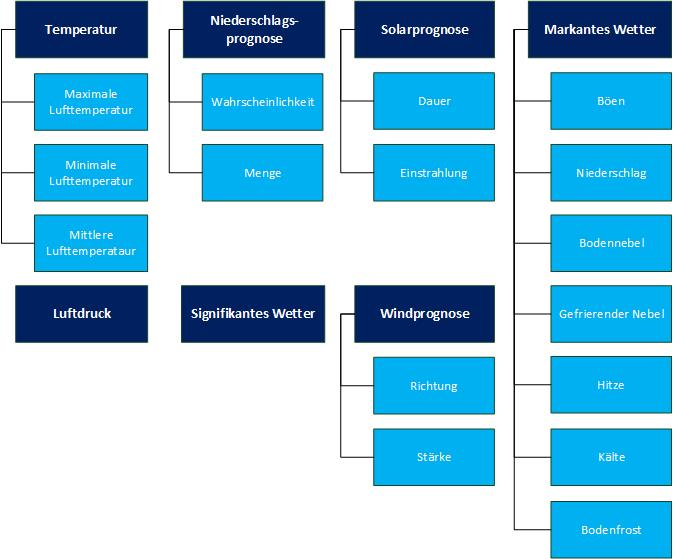
\includegraphics[scale=0.65]{weatherstation/Datenuebersicht}
\caption{Verfuegbare Prognosedaten WS-K RTU485 WPAia\cite[S. 5]{HKWDoc}}
\label{fig:1}
\end{figure}
Für welche Bereiche diese metereologischen Daten zutreffen muss in der Wetterregion spezifiziert werden. Hier besteht die Möglichkeit für über 1000 Städte in fast ganz Europa die Wetterprognosen abzufragen\cite[S. 27-38]{HKWDoc}. Wie schon in der Einleitung erwähnt, wäre eine niedrige zeitliche Auflösung der Daten wünschenswert, damit das Energiemanagementsystem ohne große Verwerfungen planen kann. Jedoch liegen die meisten Daten in einer Auflösung von 6 Stunden vor, d.h. für ein Intervall von morgens, mittags, nachmittags und abends. Lediglich die mittlere Lufttemperatur wird in einer 1 stündigen Auflösung bereitgestellt. Dieser Umstand wird später im Programmablauf gesondert berücksichtigt. Ein Update der Daten erfolgt ebenfalls alle 6 Stunden. Neben der Auflösung unterscheidet sich auch der Prognosehorizont innerhalb der zugänglichen Daten. Die Spanne reicht von einem bis zu drei Folgetagen. Für den aktuellen Tag, liegen für alle Bereiche Daten vor. Welche metereologische Ausprägung welche Eigenschaften besitzt, kann in der Tabelle\ref{fig:detaildatenstruktur} im Anhang nachvollzogen werden.    
\section{Technischer Aufbau der Station}
\subsection{Senderauswahl und Stationsaufbau}
Die eingesetzte Wetterstation erhält ihre Daten via Langwelle von drei auswählbaren Sendern:
\begin{itemize}
\item Sender Mainflingen DCF 49
\item Sender Burg DCF 39
\item Sender Lakihegy HGA 22 (Ungarn)
\end{itemize}
\begin{figure}[h]
\centering
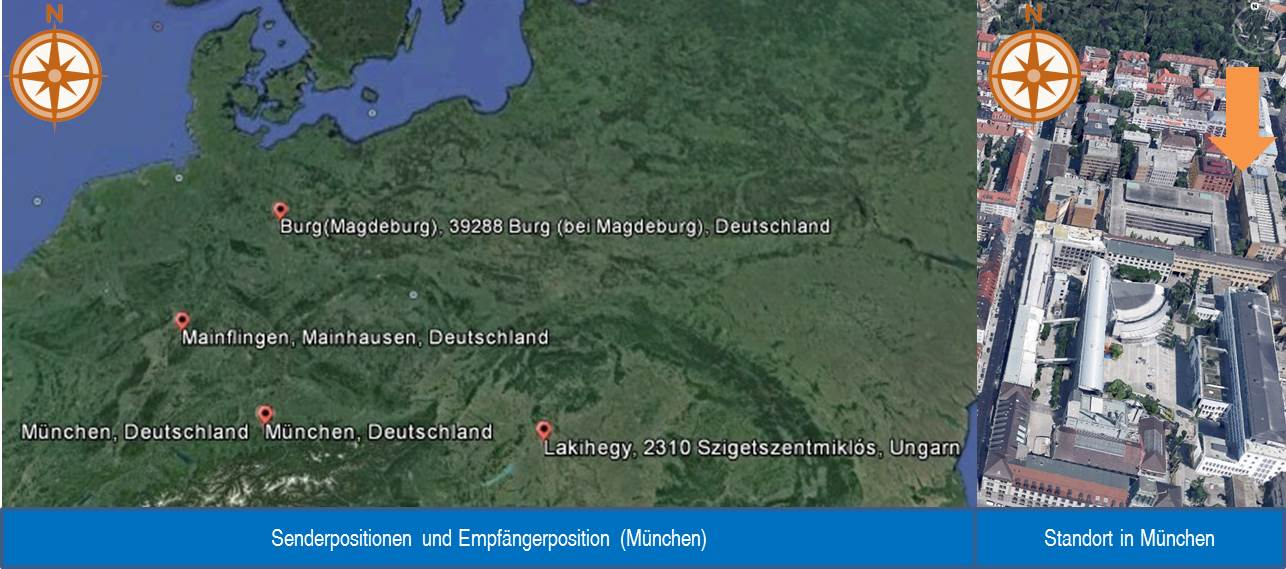
\includegraphics[scale=0.65]{weatherstation/Empfaengerausrichtung}
\caption{Standorte der Langwellensender und des Empfängers\cite[S. 15]{HKWDoc}}
\label{fig:3}
\end{figure}
Die Wetterstation soll in München aufgebaut werden. Um einen guten Empfang gewährleisten zu können, muss sie entsprechend ausgerichtet werden. Der Hersteller gibt hierzu Kriterien vor, die beachtet werden sollten\cite[S. 13 u. 15]{HKWDoc}:
\begin{itemize}
\item senkrechter Aufbau des Gehäuses mit nach unten austretendem Kabelstrang
\item für einen Innenaufbau in der Nähe zum Fenster
\item Mindestabstand von 30 cm zu Metallkonstruktionen oder -flächen
\item ausreichende Entfernung zu Geräten die elektromagnetisch abstrahlen
\item keine direkte Sonnenbestrahlung für das Einbinden der lokalen Temperatur
\item ausreichender Bodenabstand, um Einschneien zu vermeiden
\item Ausrichtung zum geografisch günstigsten Sender
\end{itemize} 
Unter Berücksichtigung dieser Empfehlungen wurde die Station in Fensternähe in nordwestlicher Richtung aufgebaut und die Sendestation Mainflingen vorgegeben.
\subsection{Registereinteilung und Schnittstellenparametrierung}
Wie im vorigen Kapitel bereits erläutert, können über das MODBUS Protokoll vier Arten von Registern angesprochen werden. In der Wetterstation sind zwei Register für die Kommunikation vorgesehen. Im Holdingregister können Einstellungsparameter gesetzt und gelesen werden. Eine Übersicht gibt die oben aufgeführte Tabelle \ref{tab:kommeinstpara}.
\begin{table}[t]
\rowcolors{1}{cyan}{white}
{
\setlength{\extrarowheight}{0.1cm}
\begin{tabular}{| c | l | c | l | l | p{2.5cm} |}
\hline
\textbf{\parbox[t]{2cm}{Register-\\adresse}} & \textbf{Bezug} & \textbf{Zugriff} & \textbf{Datentyp} & \textbf{Bereich} & \textbf{Bemerkung}\\[1cm]
\hline \hline
\hiderowcolors
110 & Senderstation & Lesen/Schreiben & unsigned & 0,1,2 & 0 = DCF 49 \newline 1 = HGA 22 \newline 2 = DCF 39\\
111 & Empfangsqualität & Lesen & unsigned & 0...9 & 9 ist höchste Qualität\\
112 & Stadt ID & Lesen/Schreiben & unsigned & 0...1022 & \\
100 & Sekunde (Funkuhr) & Lesen & unsigned & & UTC\\ 
101 & Minute (Funkuhr) & Lesen & unsigned & & UTC\\
102 & Stunde (Funkuhr) & Lesen & unsigned & & UTC\\
103 & Tag (Funkuhr) & Lesen & unsigned & & UTC\\
104 & Monat (Funkuhr) & Lesen & unsigned & & UTC\\
105 & Jahr (Funkuhr) & Lesen & unsigned & & UTC\\
\hline
\end{tabular}
}
\caption{Einstellungsparameter für den Kommunikationsaufbau und den Wetterbereich \cite[S. 16-17]{HKWDoc}}
\label{tab:kommeinstpara}
\end{table} 
Außerdem sind sämtliche metereologischen Daten in diesem Register abgelegt. Eine Auflistung der den Prognosebereichen zugeordneten Registeradressen gibt die im Anhang befindliche Tabelle\ref{fig:detaildatenstruktur}. Es ist dabei zu beachten, dass die Adressen gegenüber den in der Spezifikation des Herstellers Angegebenen, bereits auf die Struktur des Holdingregisters angepasst wurden. D.h. da das Holdingregister mit einer 0 beginnt, wurde von jeder Adresse eine Position abgezogen. Neben dem Holdingregister gibt es noch das Coilregister, in welchem die Zustände für den externen Temperatursensor und die FSK Qualität vorgehalten werden. Die Adressen hierfür sind 1 bzw. 2 und die zugelassenen Werte 1 und 0 geben jeweils den Zustand an. 1 bedeutet der Sensor sowie die FSK Qualität sind in Ordnung. 


    

\chapter{Funktionscode Dokumentation}
\chapter{Datenanalyse}
\part{Schluss}
\noindent Hiermit erkläre ich,\\
Name: Henneberger\\
Vorname: Andreas Helmut\\
Mat.Nr.: 2647351\vspace{0.4cm}\\
dass ich die beiliegende Bachelor's Thesis zum Thema:\vspace{0.5cm}\\
\begin{center}
\textbf{Aufbau einer Schnittstelle zwischen Matlab und einer Wetterstation über MODBUS}
\end{center}\vspace{0.4cm}
selbständig verfasst, keine anderen als die angegebenen Quellen und Hilfsmittel benutzt habe,
sowie alle wörtlichen und sinngemäß übernommenen Stellen in der Arbeit gekennzeichnet und die 
entsprechenden Quellen angegeben habe.\\
Vom Lehrstuhl und seinen Mitarbeitern zur Verfügung gestellte Hilfsmittel, wie Modelle oder
Programme, sind ebenfalls angegeben. Diese Hilfsmittel sind Eigentum des Lehrstuhls bzw. des
jeweiligen Mitarbeiters. Ich werde sie nicht über die vorliegende Arbeit hinaus weiter verwenden
oder an Dritte weitergeben.\vspace{0.5cm}\\

\noindent Einer weiteren Nutzung dieser Arbeit und deren Ergebnisse (auch Programme und Methoden) zu Zwecken
der Forschung und Lehre, stimme ich zu.\vspace{0.5cm}\\

\noindent Ich habe diese Arbeit noch nicht zum Erwerb eines anderen Leistungsnachweises eingereicht.\vspace{0.5cm}\\

\noindent München, \date{\today}\vspace{0.5cm}\\
\noindent ...........................................\\
Andreas Henneberger
\appendix
\renewcommand*{\appendixpagename}{Anhang}
\renewcommand*{\appendixtocname}{Anhang}
\appendixpage 
\addappheadtotoc
\chapter{Aufbau der Wetterstation} 
%\begin{figure}[h]
%\centering
%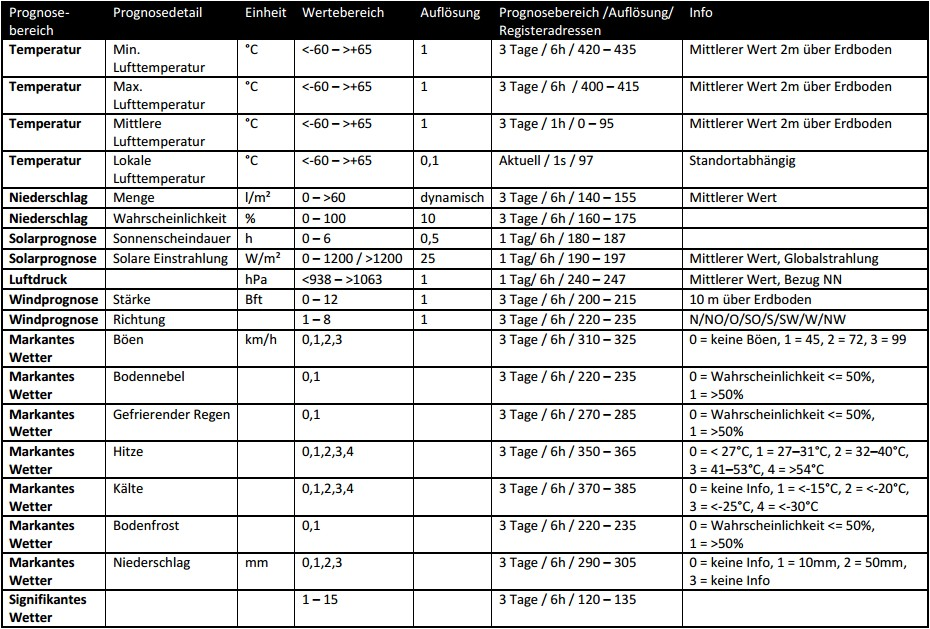
\includegraphics[scale=0.65]{weatherstation/TabDatenstruktur}
%\caption{Detailierte Datenstruktur der Wetterstation\cite[S. 17-26]{HKWDoc}}
%\label{fig:detaildatenstruktur}
%\end{figure}
\begin{table}[!b]
\rotatebox{90}{
\begin{minipage}[!b]{\textwidth}
\resizebox{18.9cm}{!}{ 
\rowcolors{1}{cyan}{white}
{
\setlength{\extrarowheight}{0.1cm}
\begin{tabular}[!b]{| p{2.5cm} | l | l | l | l | l | l | l | p{6.4cm} |}
\hline
\textbf{\parbox[t]{2.7cm}{Prognose-\\Bereich}} & \textbf{Prognosedetail} & \textbf{\parbox[t]{1.2cm}{Ein-\\heit}} & \textbf{Wertebereich} & \textbf{\parbox[t]{1.7cm}{Auf-\\lösung}} & \textbf{\parbox[t]{1.95cm}{Prognose-\\intervall}} & \textbf{\parbox[t]{1.9cm}{zeitliche\\Auflösung}} & \textbf{\parbox[t]{1.9cm}{Register-\\adresse}} & \textbf{Info}\\[1cm]
%\textbf{\parbox[t]{2cm}{Prognose-\\bereich}} & \textbf{Prognosedetail} & \textbf{Einheit} & \textbf{Wertebereich} & \textbf{Aufloesung} & \textbf{Prognoseintervall} & \textbf{zeitliche Aufloesung} & \textbf{Registeradresse} & \textbf{Info}\\[1cm]
\hline \hline
\hiderowcolors
Temperatur & Min. Lufttemperatur & $^\circ$C &  $<-60$ bis $>65$ & 1 & 3 Tage & 6h & 420 - 435 & Mittlerer Wert 2m über Erdboden\\
Temperatur & Max. Lufttemperatur & $^\circ$C &  $<-60$ bis $>65$ & 1 & 3 Tage & 6h & 400 - 415 & Mittlerer Wert 2m über Erdboden\\
Temperatur & Mittlere Lufttemperatur & $^\circ$C &  $<-60$ bis $>65$ & 1 & 3 Tage & 1h & 000 - 095 & Mittlerer Wert 2m über Erdboden\\
Temperatur & Lokale Lufttemperatur & $^\circ$C &  $<-60$ bis $>65$ & 1 & Aktuell & 1s & 097 & Standortabhängig\\
Niederschlag & Menge & l/m$^2$ &  0-60 & dyn. & 3 Tage & 6h & 140 - 155 & Mittlerer Wert\\
Niederschlag & Wahrscheinlichkeit & \% &  0 - 100 & 10 & 3 Tage & 6h & 160 - 175 & \\
Solarprognose & Sonnenscheindauer & h &  0 - 6 & 1 & 1 Tag & 6h & 180 - 187 & Mittlerer Wert\\
Solarprognose & Solare Einstrahlung & W/m$^2$ &  0 – 1200/$>1200$ & 25 & 1 Tag & 6h & 190 - 197 & Mittlerer Wert Globalstrahlung\\
Luftdruck & Min. Lufttemperatur & hPa &  $<938$ – $>1063$ & 1 & 1 Tag & 6h & 240 - 247 & Mittlerer Wert bezogen auf NN\\
Windprognose & Stärke & Bft &  0 - 12 & 1 & 3 Tage & 6h & 200 - 215 & Mittlerer Wert 10m über Erdboden\\
Windprognose & Richtung &  &  1 - 8 & 1 & 3 Tage & 6h & 220 - 235 & N/NO/O/SO/S/SW/W/NW\\
Markantes Wetter & Böen &  &  0,1,2,3 & 1 & 3 Tage & 6h & 310 - 325 & 0=keine Böen, 1=45km/h, 2=72km/h, 3=99km/h \\
Markantes Wetter & Bodennebel &  & 0,1 & 1 & 3 Tage & 6h & 250 - 265 & 0=Wahrscheinlichkeit$<=$50\%, 1=$>$50\%\\
Markantes Wetter & Gefrierender Regen &  & 0,1 & 1 & 3 Tage & 6h & 270 - 285 & 0=Wahrscheinlichkeit$<=$50\%,1=$>$50\%\\
Markantes Wetter & Hitze & $^\circ$C &  0,1,2,3,4 & 1 & 3 Tage & 6h & 350 - 365 & 0=$<$27$^\circ$C, 1=27–31$^\circ$C, 2=32–40$^\circ$C, 3=41–53$^\circ$C, 4=$>$54$^\circ$C\\
Markantes Wetter & Kälte & $^\circ$C &  0,1,2,3,4 & 1 & 3 Tage & 6h & 370 - 385 & 0=keine Info, 1=$<$-15$^\circ$C, 2=$<$-20$^\circ$C, 3=$<$-25$^\circ$C, 4=$<$-30$^\circ$C\\
Markantes Wetter & Bodenfrost &  &  0,1 & 1 & 3 Tage & 6h & 290 - 305 & 0=Wahrscheinlichkeit$<=$50\%, 1=$>$50\%\\
Markantes Wetter & Niederschlag &  &  0,1,2,3 & 1 & 3 Tage & 6h & 330 - 345 & 0=keine Info, 1=10mm, 2=50mm, 3=keine Info\\
Signifikantes Wetter &  &  & 1 - 15 & 1 & 3 Tage & 6h & 120 - 135 & 1=sonnig/klar, 2=leicht bewölkt, 3=vorwiegend bewölkt, 4=bedeckt, 5=Wärmegewitter, 6=starker Regen, 7=Schneefall, 8=Nebel, 9=Schneeregen, 10=Regenschauer, 11=leichter Regen, 12=Schneeschauer, 13=Frontengewitter, 14=Hochnebel, 15=Schneeregenschauer\\
\hline
\end{tabular}
}
}
\caption{Detailierte Datenstruktur der Wetterstation\cite[S. 17-26]{HKWDoc}}
\label{tab:detaildatenstruktur}
\end{minipage}
}
\end{table}
\FloatBarrier
\chapter{Das MODBUS Protokoll}
\begin{figure}[h]
\centering
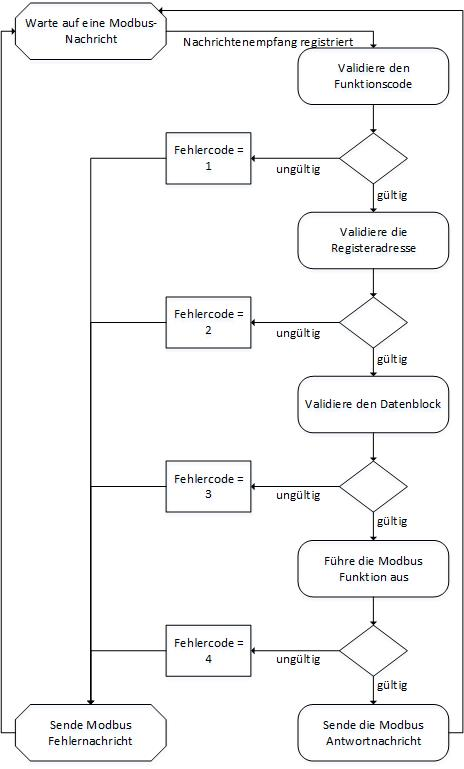
\includegraphics[scale=0.65]{modbus/modbustransdiag}
\caption{Ablaufdiagramm für die MODBUS Nachrichtenüberprüfung}
\label{fig:modbustransdiag}
\end{figure}
\newpage
\begin{figure}[hbtp]
\centering
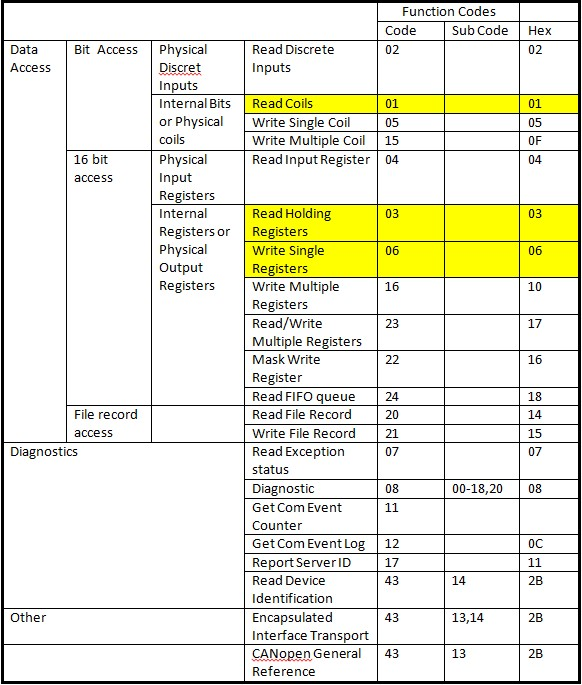
\includegraphics[scale=0.65]{modbus/fcodetab}
\caption{Übersicht der zur Verfügung stehenden Funktionscodes in MODBUS}
\label{fig:fcodetab}
\end{figure} 
\chapter{Abkürzungsverzeichnis}
\begin{acronym}
\setlength{\parskip}{0ex}
\setlength{\itemsep}{1ex}
 \acro{ADU}{Application Data Unit}
 \acro{Bft}{Beaufort}
 \acro{C}{Celsius}
 \acro{COM}{Communication}
 \acro{CRC}{Cyclic Redundancy Check}
 \acro{DWD}{Deutscher Wetterdienst}
 \acro{EMU}{Energy Management Unit}
 \acro{EV}{Electric Vehicle}
 \acro{FSK}{Frequency Shift Keying}
 \acro{GmbH}{Gesellschaft mit beschränkter Haftung}
 \acro{h}{Stunde}
 \acro{hPa}{Hektopascal}
 \acro{HEMS}{Home Energy Management System}
 \acro{H-Byte}{High-Byte}
 \acro{ID}{Identifkationsnummer}
 \acro{int8}{8 Bit-Integer}
 \acro{IP}{Internet Protocol}
 \acro{I/O}{Input/Output}
 \acro{LMU}{Ludwig-Maximilians-Universität}
 \acro{L-Byte}{Low-Byte}
 \acro{N}{Nord}
 \acro{NN}{Normal Null Meeresspiegel}
 \acro{NO}{Nordost}
 \acro{NW}{Nordwest}
 \acro{O}{Osten}
 \acro{OSI}{Open Systems Interconnection}
 \acro{PDU}{Protocol Data Unit}
 \acro{RMSE}{Root mean square error}
 \acro{RS}{Recommended Standard}
 \acro{RTU}{Remute Terminal Unit}
 \acro{rx}{Empfänger}
 \acro{TCP}{Transmission Control Protocol}
 \acro{S}{Sueden}
 \acro{SO}{Suedost}
 \acro{SW}{Suedwest}
 \acro{W}{Westen}
\end{acronym}

\bibliographystyle{unsrt} 
\bibliography{literatur} 

\end{document}


